\begin{figure}[p]\centering
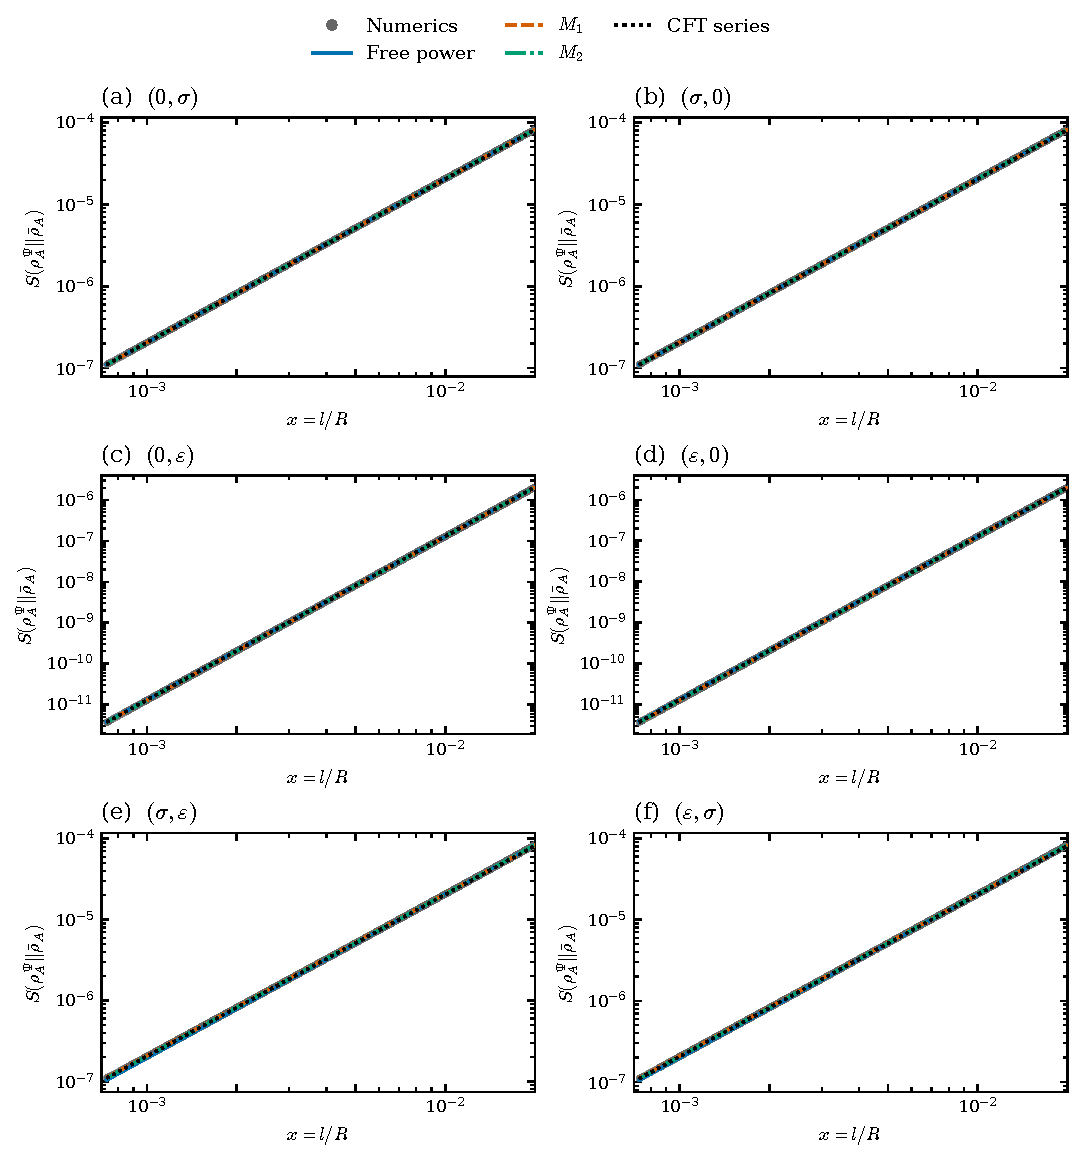
\includegraphics[width=.94\linewidth,height=.74\textheight,keepaspectratio]{figs/ising_small_fit_window_value.pdf}
\caption{Ising small-interval $D^A_{a\mid b}$ for all six ordered pairs. All 1255 displayed geometries per direction lie in the fitting window $0<x\leq0.02$, with $\ell=6,\ldots,10$. Both axes are logarithmic. Gray circles denote numerical data, using the same shape and color for every subsystem length. Blue solid, orange dashed, and green dash--dotted curves denote the free fit, $F_1$, and $F_2$; black dotted denotes the parameter-free CFT series. All curves are restricted to the fitting window.}
\label{fig:num-ising-small}
\end{figure}

\begin{figure}[p]\centering
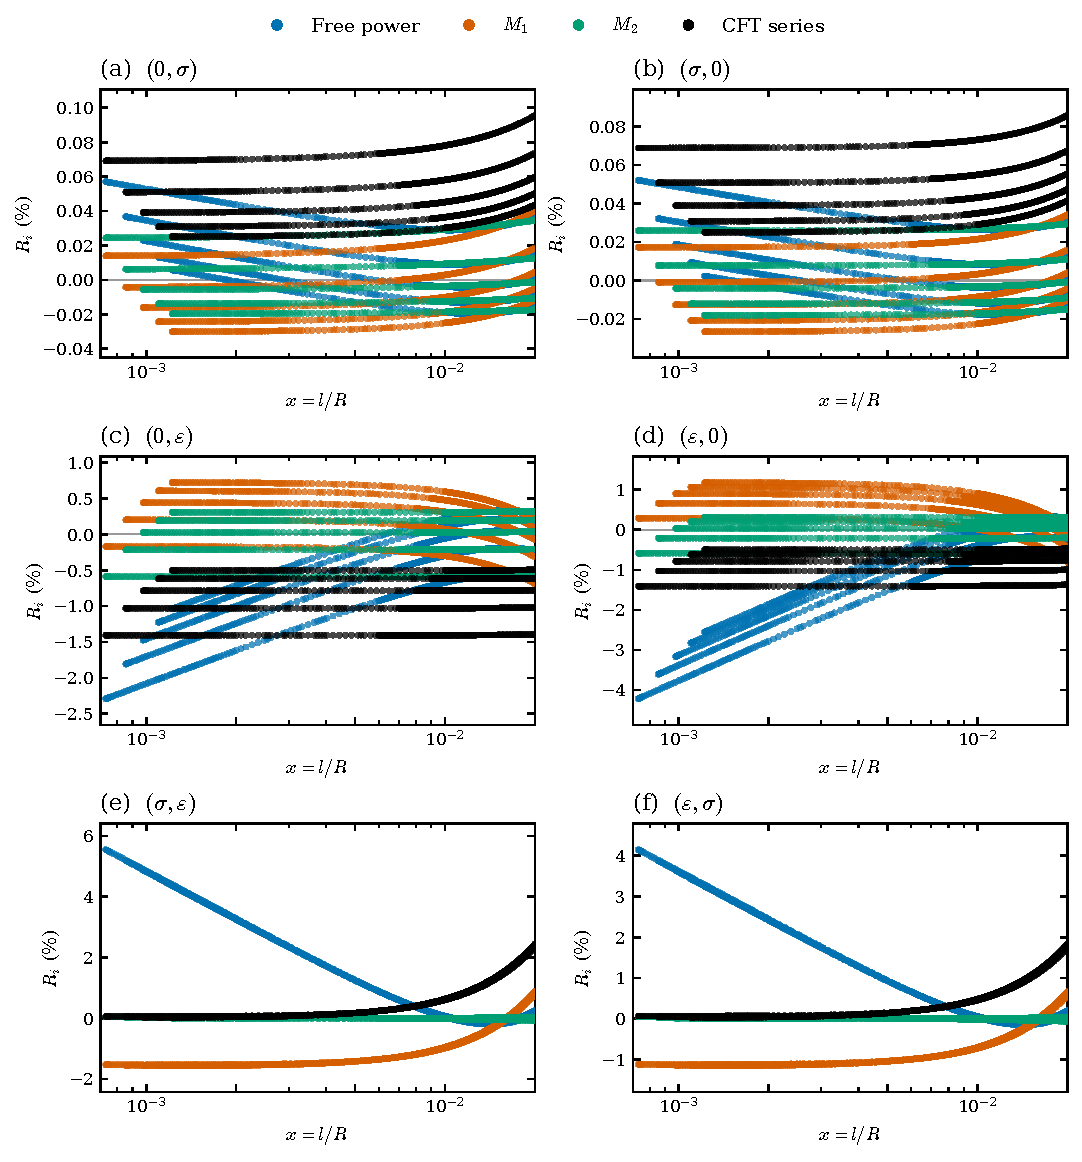
\includegraphics[width=.94\linewidth,height=.74\textheight,keepaspectratio]{figs/ising_small_fit_window_residual.pdf}
\caption{Signed percentage residuals $100[q-M]/q$ for Fig.~\ref{fig:num-ising-small}, with $q=D^A$. The residual ordinate is linear and the fraction axis logarithmic. Only the 1255 fitted geometries per direction at $0<x\leq0.02$ are shown. All subsystem lengths $\ell=6,\ldots,10$ use circular markers; colors identify models and are identical across lengths. Blue, orange, green, and black denote the free fit, $F_1$, $F_2$, and the parameter-free CFT series.}
\label{fig:num-ising-small-residual}
\end{figure}
